\documentclass{standalone}
\usepackage{tikz}
\usetikzlibrary{patterns, positioning}


\begin{document}
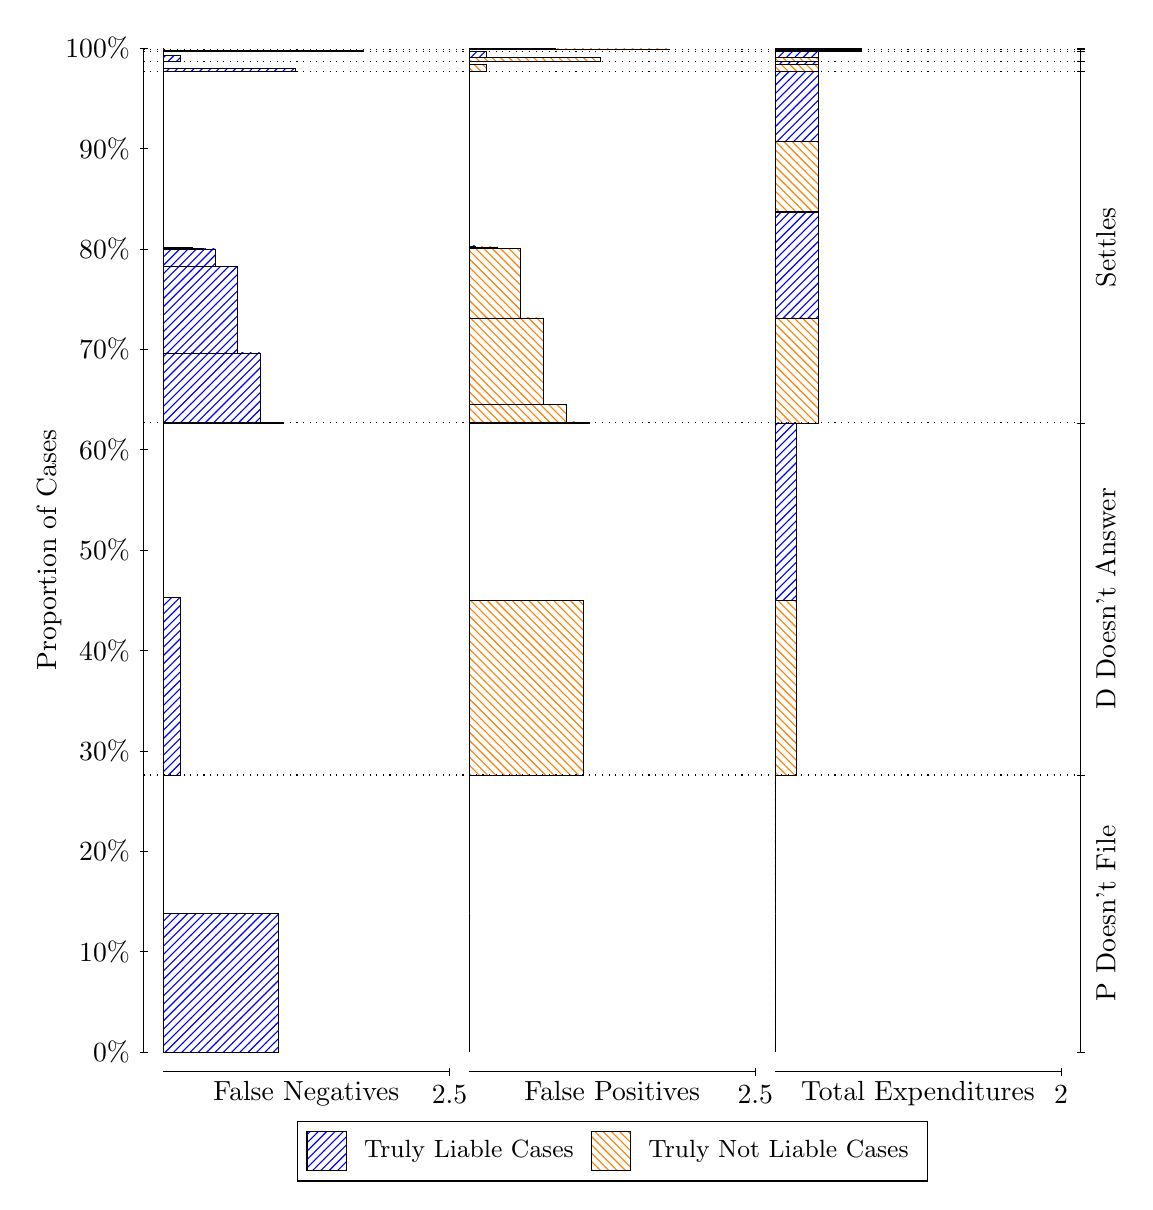
\begin{tikzpicture}
\draw[black, very thin] (1.5,1.75) -- (1.5,14.5);
\node[rotate=90, text=black, anchor=center] at (0.3, 8.125) {Proportion of Cases};
\draw[black, very thin] (1.45,1.75) -- (1.55,1.75);
\node[text=black, anchor=east] at (1.45, 1.75) {0\%};
\draw[black, very thin] (1.45,3.025) -- (1.55,3.025);
\node[text=black, anchor=east] at (1.45, 3.025) {10\%};
\draw[black, very thin] (1.45,4.3) -- (1.55,4.3);
\node[text=black, anchor=east] at (1.45, 4.3) {20\%};
\draw[black, very thin] (1.45,5.575) -- (1.55,5.575);
\node[text=black, anchor=east] at (1.45, 5.575) {30\%};
\draw[black, very thin] (1.45,6.85) -- (1.55,6.85);
\node[text=black, anchor=east] at (1.45, 6.85) {40\%};
\draw[black, very thin] (1.45,8.125) -- (1.55,8.125);
\node[text=black, anchor=east] at (1.45, 8.125) {50\%};
\draw[black, very thin] (1.45,9.4) -- (1.55,9.4);
\node[text=black, anchor=east] at (1.45, 9.4) {60\%};
\draw[black, very thin] (1.45,10.675) -- (1.55,10.675);
\node[text=black, anchor=east] at (1.45, 10.675) {70\%};
\draw[black, very thin] (1.45,11.95) -- (1.55,11.95);
\node[text=black, anchor=east] at (1.45, 11.95) {80\%};
\draw[black, very thin] (1.45,13.225) -- (1.55,13.225);
\node[text=black, anchor=east] at (1.45, 13.225) {90\%};
\draw[black, very thin] (1.45,14.5) -- (1.55,14.5);
\node[text=black, anchor=east] at (1.45, 14.5) {100\%};

\draw[black, very thin] (13.4,1.75) -- (13.4,14.5);
\draw[black, very thin] (13.35,1.75) -- (13.45,1.75);
\node[anchor=west] at (13.35, 1.75) {};
\draw[black, very thin] (13.35,5.2672) -- (13.45,5.2672);
\node[anchor=west] at (13.35, 5.2672) {};
\draw[black, very thin] (13.35,9.7407) -- (13.45,9.7407);
\node[anchor=west] at (13.35, 9.7407) {};
\draw[black, very thin] (13.35,14.199) -- (13.45,14.199);
\node[anchor=west] at (13.35, 14.199) {};
\draw[black, very thin] (13.35,14.331) -- (13.45,14.331);
\node[anchor=west] at (13.35, 14.331) {};
\draw[black, very thin] (13.35,14.461) -- (13.45,14.461);
\node[anchor=west] at (13.35, 14.461) {};
\draw[black, very thin] (13.35,14.481) -- (13.45,14.481);
\node[anchor=west] at (13.35, 14.481) {};
\draw[black, very thin] (13.35,14.5) -- (13.45,14.5);
\node[anchor=west] at (13.35, 14.5) {};

\draw[black, very thin, pattern color=blue, pattern=north east lines] (1.75,1.75) rectangle (3.2033,3.5086);
\draw[black, very thin, pattern color=orange, pattern=north west lines] (1.75,3.5086) rectangle (1.75,5.2672);
\draw[black, very thin, pattern color=blue, pattern=north east lines] (1.75,5.2672) rectangle (1.968,7.5213);
\draw[black, very thin, pattern color=orange, pattern=north west lines] (1.75,7.5213) rectangle (1.75,9.7407);
\draw[black, very thin, pattern color=blue, pattern=north east lines] (1.75,9.7407) rectangle (3.276,9.7438);
\draw[black, very thin, pattern color=blue, pattern=north east lines] (1.75,9.7438) rectangle (3.1307,9.7474);
\draw[black, very thin, pattern color=blue, pattern=north east lines] (1.75,9.7474) rectangle (2.9853,10.627);
\draw[black, very thin, pattern color=blue, pattern=north east lines] (1.75,10.627) rectangle (2.84,10.627);
\draw[black, very thin, pattern color=blue, pattern=north east lines] (1.75,10.627) rectangle (2.6947,11.727);
\draw[black, very thin, pattern color=blue, pattern=north east lines] (1.75,11.727) rectangle (2.5493,11.727);
\draw[black, very thin, pattern color=blue, pattern=north east lines] (1.75,11.727) rectangle (2.404,11.948);
\draw[black, very thin, pattern color=blue, pattern=north east lines] (1.75,11.948) rectangle (2.2587,11.953);
\draw[black, very thin, pattern color=blue, pattern=north east lines] (1.75,11.953) rectangle (2.1133,11.966);
\draw[black, very thin, pattern color=orange, pattern=north west lines] (1.75,11.966) rectangle (1.75,14.199);
\draw[black, very thin, pattern color=blue, pattern=north east lines] (1.75,14.199) rectangle (3.4213,14.242);
\draw[black, very thin, pattern color=orange, pattern=north west lines] (1.75,14.242) rectangle (1.75,14.331);
\draw[black, very thin, pattern color=blue, pattern=north east lines] (1.75,14.331) rectangle (1.968,14.406);
\draw[black, very thin, pattern color=orange, pattern=north west lines] (1.75,14.406) rectangle (1.75,14.461);
\draw[black, very thin, pattern color=blue, pattern=north east lines] (1.75,14.461) rectangle (4.2933,14.468);
\draw[black, very thin, pattern color=orange, pattern=north west lines] (1.75,14.468) rectangle (1.75,14.481);
\draw[black, very thin, pattern color=orange, pattern=north west lines] (1.75,14.481) rectangle (1.75,14.488);
\draw[black, very thin, pattern color=blue, pattern=north east lines] (1.75,14.488) rectangle (1.75,14.5);
\draw[black, very thin, pattern color=orange, pattern=north west lines] (5.6333,1.75) rectangle (5.6333,3.5086);
\draw[black, very thin, pattern color=blue, pattern=north east lines] (5.6333,3.5086) rectangle (5.6333,5.2672);
\draw[black, very thin, pattern color=orange, pattern=north west lines] (5.6333,5.2672) rectangle (7.0867,7.4866);
\draw[black, very thin, pattern color=blue, pattern=north east lines] (5.6333,7.4866) rectangle (5.6333,9.7407);
\draw[black, very thin, pattern color=orange, pattern=north west lines] (5.6333,9.7407) rectangle (7.1593,9.7454);
\draw[black, very thin, pattern color=orange, pattern=north west lines] (5.6333,9.7454) rectangle (7.014,9.7509);
\draw[black, very thin, pattern color=orange, pattern=north west lines] (5.6333,9.7509) rectangle (6.8687,9.9714);
\draw[black, very thin, pattern color=orange, pattern=north west lines] (5.6333,9.9714) rectangle (6.7233,9.9715);
\draw[black, very thin, pattern color=orange, pattern=north west lines] (5.6333,9.9715) rectangle (6.578,11.072);
\draw[black, very thin, pattern color=orange, pattern=north west lines] (5.6333,11.072) rectangle (6.4327,11.072);
\draw[black, very thin, pattern color=orange, pattern=north west lines] (5.6333,11.072) rectangle (6.2873,11.952);
\draw[black, very thin, pattern color=orange, pattern=north west lines] (5.6333,11.952) rectangle (6.142,11.96);
\draw[black, very thin, pattern color=orange, pattern=north west lines] (5.6333,11.96) rectangle (5.9967,11.974);
\draw[black, very thin, pattern color=blue, pattern=north east lines] (5.6333,11.974) rectangle (5.706,11.986);
\draw[black, very thin, pattern color=blue, pattern=north east lines] (5.6333,11.986) rectangle (5.6333,14.199);
\draw[black, very thin, pattern color=orange, pattern=north west lines] (5.6333,14.199) rectangle (5.8513,14.288);
\draw[black, very thin, pattern color=blue, pattern=north east lines] (5.6333,14.288) rectangle (5.6333,14.331);
\draw[black, very thin, pattern color=orange, pattern=north west lines] (5.6333,14.331) rectangle (7.3047,14.386);
\draw[black, very thin, pattern color=blue, pattern=north east lines] (5.6333,14.386) rectangle (5.8513,14.461);
\draw[black, very thin, pattern color=orange, pattern=north west lines] (5.6333,14.461) rectangle (5.6333,14.474);
\draw[black, very thin, pattern color=blue, pattern=north east lines] (5.6333,14.474) rectangle (5.6333,14.481);
\draw[black, very thin, pattern color=orange, pattern=north west lines] (5.6333,14.481) rectangle (8.1767,14.488);
\draw[black, very thin, pattern color=blue, pattern=north east lines] (5.6333,14.488) rectangle (6.7233,14.5);
\draw[black, very thin, pattern color=orange, pattern=north west lines] (9.5167,1.75) rectangle (9.5167,3.5086);
\draw[black, very thin, pattern color=blue, pattern=north east lines] (9.5167,3.5086) rectangle (9.5167,5.2672);
\draw[black, very thin, pattern color=orange, pattern=north west lines] (9.5167,5.2672) rectangle (9.7892,7.4866);
\draw[black, very thin, pattern color=blue, pattern=north east lines] (9.5167,7.4866) rectangle (9.7892,9.7407);
\draw[black, very thin, pattern color=orange, pattern=north west lines] (9.5167,9.7407) rectangle (10.062,11.072);
\draw[black, very thin, pattern color=blue, pattern=north east lines] (9.5167,11.072) rectangle (10.062,12.41);
\draw[black, very thin, pattern color=orange, pattern=north west lines] (9.5167,12.41) rectangle (10.062,12.424);
\draw[black, very thin, pattern color=blue, pattern=north east lines] (9.5167,12.424) rectangle (10.062,12.428);
\draw[black, very thin, pattern color=orange, pattern=north west lines] (9.5167,12.428) rectangle (10.062,13.316);
\draw[black, very thin, pattern color=blue, pattern=north east lines] (9.5167,13.316) rectangle (10.062,14.199);
\draw[black, very thin, pattern color=orange, pattern=north west lines] (9.5167,14.199) rectangle (10.062,14.288);
\draw[black, very thin, pattern color=blue, pattern=north east lines] (9.5167,14.288) rectangle (10.062,14.331);
\draw[black, very thin, pattern color=orange, pattern=north west lines] (9.5167,14.331) rectangle (10.062,14.386);
\draw[black, very thin, pattern color=blue, pattern=north east lines] (9.5167,14.386) rectangle (10.062,14.461);
\draw[black, very thin, pattern color=orange, pattern=north west lines] (9.5167,14.461) rectangle (10.607,14.474);
\draw[black, very thin, pattern color=blue, pattern=north east lines] (9.5167,14.474) rectangle (10.607,14.481);
\draw[black, very thin, pattern color=orange, pattern=north west lines] (9.5167,14.481) rectangle (10.607,14.488);
\draw[black, very thin, pattern color=blue, pattern=north east lines] (9.5167,14.488) rectangle (10.607,14.5);
\draw[black, dotted] (1.5,5.2672) -- (13.4,5.2672);
\draw[black, dotted] (1.5,9.7407) -- (13.4,9.7407);
\draw[black, dotted] (1.5,14.199) -- (13.4,14.199);
\draw[black, dotted] (1.5,14.331) -- (13.4,14.331);
\draw[black, dotted] (1.5,14.461) -- (13.4,14.461);
\draw[black, dotted] (1.5,14.481) -- (13.4,14.481);
\draw[black, very thin] (1.75,1.5) -- (5.3833,1.5);
\node[text=black, anchor=north] at (3.5667, 1.5) {False Negatives};
\draw[black, very thin] (5.3833,1.45) -- (5.3833,1.55);
\node[text=black, anchor=north] at (5.3833, 1.45) {2.5};

\draw[black, very thin] (5.6333,1.5) -- (9.2667,1.5);
\node[text=black, anchor=north] at (7.45, 1.5) {False Positives};
\draw[black, very thin] (9.2667,1.45) -- (9.2667,1.55);
\node[text=black, anchor=north] at (9.2667, 1.45) {2.5};

\draw[black, very thin] (9.5167,1.5) -- (13.15,1.5);
\node[text=black, anchor=north] at (11.333, 1.5) {Total Expenditures};
\draw[black, very thin] (13.15,1.45) -- (13.15,1.55);
\node[text=black, anchor=north] at (13.15, 1.45) {2};

\node[text=black, centered, rotate=90] at (13.72, 3.5086) {P Doesn't File};
\node[text=black, centered, rotate=90] at (13.72, 7.504) {D Doesn't Answer};
\node[text=black, centered, rotate=90] at (13.72, 11.97) {Settles};





\draw (7.449999999999999,1.5) node[draw=none] (baseCoordinate) {};
\begin{scope}[align=center]
        \matrix[scale=0.5, draw=black, below=0.5cm of baseCoordinate, nodes={draw}, column sep=0.1cm]{
            \node[rectangle, draw, minimum width=0.5cm, minimum height=0.5cm, pattern color=blue, pattern=north east lines] {}; &
            \node[draw=none, font=\small, text=black] (B) {Truly Liable Cases}; &
            \node[rectangle, draw, minimum width=0.5cm, minimum height=0.5cm, pattern color=orange, pattern=north west lines] {}; &
            \node[draw=none, font=\small, text=black] (B) {Truly Not Liable Cases}; \\
            };
\end{scope}

\end{tikzpicture}
\end{document}